\documentclass[__main__.tex]{subfiles}

\begin{document}

\section{Теорема Лакса для схемы табличных аналогов линейного уравнения с единственным решением в сепарабельном банаховом пространстве}

Если схема
\begin{gather}
\label{8.1}
\begin{cases}
\underline{F}_{(k)} \cdot ^{>} \underline{u}_{(k)} = ^{>}\underline{v}_{(k)} = \hat{\pi}_{k} (y_0),\\
k \to +\infty
\end{cases}
\end{gather}
аппроксимирует уравнение $\hat{F}(x) = y_0$ и устойчива, то схема \ref{8.1} корректна, т.е. аналетически корректна.\\
$\lim \hat{\phi_k} \circ \underline{\hat{F}}_{(k)}^{-1} \circ \hat{\pi}_{k} (y_0) = x_0$ - решение $\hat{F}(x) = y_0$ и устойчива, т.е. $|| \hat{\phi}_{k} \circ \underline{\hat{F}}_{(k)}^{-1} \circ \hat{\pi}_k|| \leq const$ для $\forall k \in N$ (const не зависит от k).\\

\begin{proof}
Поскольку уравнение $\hat{F}(x) = y_0$ имело единственное решение $x_0 \in D(\hat{F}) = X_0$, то для $k \in N$ рассмотрим:\\
$\hat{\pi}_k$ - табличную функцию $\hat{\pi}_k(x_0) \in ^{>} R_{*}^{k+1}$. Кроме того, поскольку схема таблицных аналогов \ref{8.1} - устойчива, то для каждого $k \in N \ \exists \underline{F}_{(k)}^{-1}$ и $^{>} \underline{x}_{(k)} = \underline{F}_{(k)}^{-1} \cdot \hat{\pi}_{k} (y_0)$ - решение СЛАУ:\\
$\underline{\hat{F}}_{(k)} \cdot ^{>} \underline{u}_{(k)} = \hat{\pi}_{k} (y_0)$\\

Поскольку схема \ref{8.1} апроксимирует уравнение $\hat{F}(x) = y_0$, то:\\
\begin{gather}
\label{8.2}
\begin{cases}
F_{(k)} \cdot \hat{\pi}_{k} (x_0) = \hat{\pi}_k (y_0) + ^{>} \underline{\epsilon}_{(k)} \text{для} k \in N,\\
\lim_{k \to +\infty} ||^{>} \underline{\epsilon}_{(k)}|| = 0 
\end{cases}
\end{gather}

Таким образом:
\begin{gather}
\begin{cases}
- \underline{F}_{(k)} \cdot ^{>} \underline{x}_{(k)} + \underline{F}_{(k)} \cdot \hat{\pi}_{k} (x_0) = - \underline{F}_{(k)} \cdot (^{>}\underline{x}_{(k)} - \hat{\pi}_{k} (x_0)) = -\hat{\pi}_{k} (y_0) + \hat{\pi}_{k} (y_0) + ^{>} \underline{\epsilon}_{k} = ^{>} \Epsilon_{k}\\
||^{>} \underline{\epsilon}_{(k)} \to 0 \text{при} k \to + \infty
\end{cases}
\end{gather}

Отсюда получаем:
\begin{gather}
\label{8.3}
\begin{cases}
\hat{\pi}_{k} (x_0) - ^{>}\underline{x}_{(k)} = \underline{F}_{(k)}^{-1} \cdot ^{>} \underline{\epsilon}_{(k)},\\
||^{>}\underline{\epsilon}_{(k)}|| \to 0 \text{при} k \to +\infty
\end{cases}
\end{gather}

В силу устойчивости схемы \ref{8.1}:\\
$||\underline{F}_{(k)}^{-1}|| \leq C$ для $\forall k \in N$\\

Тогда получаем из \ref{8.3}:\\
$|| \hat{\pi}_{k} (x_0) - ^{>}\underline{x}_{(k)}|| \leq ||\underline{F}_{(k)}^{-1}|| \cdot ||^{>} \underline{\epsilon}_{(k)} \leq C \cdot ||^{>} \underline{\epsilon}_{(k)}|| \to 0$ при $k \to + \infty$\\

Отсюда:\\
\begin{gather}
\label{8.4}
||\hat{\phi}_{k} \circ (\hat{\pi}_{k} (x_0) - ^{>} \underline{x}_{(k)})|| = ||\hat{\phi}_{k} \circ \hat{\pi}_{k} (x_0) - \hat{\phi}_{k}(^{>} \underline{x}_{(k)})|| \leq ||\hat{\phi}_{k}|| \cdot ||\hat{\pi}_{k} (x_0) - ^{>} \underline{x}_{(k)}|| \to 0 \ \text{при} k \ \to +\infty
\end{gather} 
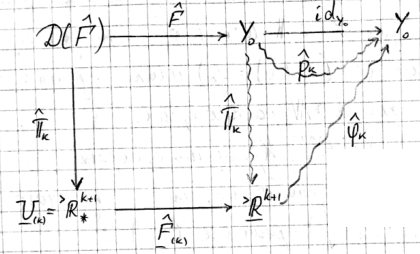
\includegraphics[width = 0.8\linewidth]{img_81}\\
т.к. $\lim_{k \to +\infty} ||\hat{\phi}_{k}|| = 1$.\\
поскольку $\hat{p}_{(\cdot)} = (\hat{p}_{k})_{N}$ - корректное апроксимирование $y_0$, то $\lim_{k \to +\infty} \hat{p}_{k} (x_0) = \lvzigzag \hat{p}_{k} = \hat{\phi}_{k} \circ \hat{\pi}_{k} \rvzigzag = \lim_{k \to +\infty} \hat{p}_{k} (x_0) = x_0$\\

Следовательно, согласно \ref{8.4}:\\
$\lim_{k \to +\infty} \hat{\phi}_{k} \circ \hat{\phi}_{k} (x_0) = \lim_{k \to +\infty} \hat{p}_{k} (x_0) = x_0 = \lim_{k \to +\infty} \hat{\phi}_{k} (^{>}x_{(k)})$,\\
где $\hat{\phi}_{k} (^{>}\underline{x}_{(k)}) = \hat{\phi}_{k} \circ \underline{\hat{F}}_{(k)}^{-1} \circ \hat{\pi}_{k} (y_0)$ -- k-ое приближенное решение уравнения $\hat{F}(x) = y_0$.\\

Таким образом, схема табличных аналогов \ref{8.1} уравнения $\hat{F}(x) = y_0$ - корректна, т.к.
$$
||\hat{\phi}_{k} \circ \underline{\hat{F}}_{(k)}^{-1} \circ \hat{\phi}_{k}||  \leq (1+\epsilon)\cdot c \cdot 1
$$
для достаточно большого $k$. (устойчивость по $y_0$).
\end{proof}
\end{document}
